
\bibliographystyle{asp2010}

\resetcounters

\markboth{Laidler and Kuttel}{Detection of Binary Pulsars}


\title{Detection of Binary Pulsars with GPU-Accelerated Sinusoidal Hough Transformations}
\author{Christopher~Laidler and Michelle~M.~Kuttel
\affil{Department of Computer Science, University of Cape Town, South Africa}
}
\aindex{Laidler, C.}
\aindex{Kuttel, M.}

\begin{abstract}
Analysis of relativistic binary pulsars is currently the best means by which to test theories of gravity in strong gravitational fields. Four-dimensional Hough Transformations can detect sinusoids in noisy images. Hough Transformations can be applied to Dynamic Power Spectra to detect the sinusoidal shift in observed spin frequency from binary pulsars in approximately circular orbits. We present four  alternative GPU implementations of a Hough Transformation algorithm, which we apply to synthesized  Dynamic Power Spectra data to determine  the GPU kernel that provides the best acceleration.
\end{abstract}

\section{Introduction}
Pulsars are highly magnetized rotating neutron stars that are observed from earth as periodic pulses across a range of frequencies. The ionized interstellar medium disperses the pulse signal over time:  we observe a pulse at higher frequencies first. Searching survey data for pulsars with \emph{a priori }unknown characteristics is known as blind searching. Standard blind search procedures scan the power spectrum (the Fourier transform of the de-dispersed survey data) and work well for periodic signals produced by solitary pulsars. However, if a pulsar is in a binary orbit, the orbital motion Doppler-shifts the observed pulse frequency, decreasing power and hindering detection.

Two methods are commonly used to search for binary pulsars. Acceleration searches assume that the orbital period is significantly longer than the observation period, allowing the simplifying assumption of a constant orbital acceleration during the observation. \citep{camilo2000observations,ransom2002fourier, Ransom2001a}. Side-band searches are used when an observation covers several complete orbits. \citep{Jouteux2002a, Ransom2003}. These two methods leave a sensitivity gap in detection of pulsars with orbital periods approximately equivalent to the duration of observation (a few hours), which is covered by the Dynamic Power Spectrum (DPS) search method. A DPS is generated by dividing the observation into short segments and calculating the power spectrum for each. These are stacked to produce a two-dimensional array in time and frequency. In a DPS, signals from pulsars in close to circular orbits appear as sinusoids. An automated search method that applies a sinusoidal Hough Transformation (HT) to a Dynamic Power Spectrum has been demonstrated to re-detect known binary pulsars in 47 Tucanae \citep{aulbert2005finding, aulbert2007finding}. While this computationally intensive method is impractical for a truly blind search, there is potential for acceleration of the Hough Transformation with commodity graphics processing units (GPUs) \citep{aulbert2005finding}. Here we use nVidia's Compute Unified Device Architecture (CUDA) to implement the sinusoidal Hough Transformation on the GPU, with the hope that a significant acceleration will allow this transformation to be integrated into existing search pipelines.

\section{The Hough Transformation}

The Hough Transformation is an image processing technique for estimation of the parameters of a parametric curve in a pixelated image. A standard Hough Transform for detecting lines of the form $y=mx+c$ will convert an $x,y$ point in image-space into a line in $m,c$-space. The intersection of two lines in parameter space represents the parameters of the line on which the two points in image space lie. With the Hough Transformation, this intersection is found by discretizing the parameter-space and counting the lines crossing a point in the discretized $mc$-space. This method is relativity insensitive to random noise and can detect features that are partially occluded or incomplete, making it a robust parameter detection method.

The polar form of the general equation of a horizontal sinusoid is given by:
\begin{equation} \label{eq:masterPolar}
y = a + p \cos\left(cx\right) - q \sin \left( cx \right ) 
\end{equation}
with $ p = b \cos\left(d\right)$ and $ q =b \sin \left( d \right)$. This is used as the master equation for the sinusoidal Hough Transformation and has four adjustable parameters: $a$, $c$, $p$ and $q$. The $a$ parameter represents the ``height'' of the sinusoid or spin frequency of the pulsar (in Hz). The $b$ parameter is the amplitude of the sinusoid and in the polar form is represented as the Euclidean distance to the $(0,0)$ point in the $p$ $q$ plain.

In general, a HT requires selecting input image pixels, calculating a hyperplane and incrementing all voxels that it intersects. Before delving into details, we make a number of observations and set conditions for an efficient implementation. For an input pixel with location $(x, y)$ and for a given value of $c$, the transformation leads to a flat 3D plain in $apq$-space. If we stipulate that $p$, $q$ and $a$ must all have the same resolution, then for a given $c$, any combination of $p$ and $q$ will lead to a unique $a$. A complete 4D hyperplane can be generated by connecting the consecutive flat 3D planes. This is easily accomplished by widening in the $a$ dimension.

\subsection{Implementations}

We developed a serial and four parallel implementations to enable method comparisons. This Hough Transformation requires many expensive trigonometric calculations, making it a complex problem to accelerate. The serial implementation uses intelligent decomposition and loop ordering and a large section of main memory to store previous calculations, to accelerate the transformation. This implementation first loops over $x$ and then $c$, performing expensive trigonometric calculations as early as possible. We next loop over the polar coordinates and the subset of $y$ which results in an $a$ values within the bounds of the tile. To create a complete 4D manifold, we fill all points between a calculated $a$ value and the $a$ value calculated from the previous $c$, which is stored in main memory. Although not done here, this CPU version is easily parallelised for multiple cores with OpenMP, using an `omp parallel for' directive on the initial loop.

We implemented four alternate CUDA kernels to perform the transformation, to evaluate different approaches. All kernels make use of CUDA atomic memory functions. Due to memory limitations, the GPU implementations cannot store large numbers of previously calculated values and thus duplicate some trigonometric calculations. This increased computation is compensated for by the large number of computational units.

The GPU1 kernel aims to minimize thread divergence by allocating a single input pixel to each CUDA thread. All the  other kernels iterate only through the input pixels that may have an effect on the tile. This requires some divergence, but decreases the overall number of calculations required. The GPU2 kernel aims to reduce calculations by ignoring voxels that fall outside the tile. GPU2 dedicates a single CUDA thread to each $p,q$ pair, each thread looping through $x$ and $c$. The GPU3 kernel was implemented to test the use of SM to store a lookup buffer for $y$ values. The final kernel GPU4 aims to use SM to remove duplication of trigonometric calculations, by allowing a thread to read the values calculated by the thread handling the adjacent $c$.

\section{Results and Discussion}
\label{eval}

For testing, we generated synthetic DPS data, consisting of normally distributed noise with an added sinusoidal signal. While the transforms successfully detect the sinusoidal signal in the input images, we do not discuss the power of the transform here. We focus on the speed of the transformations, measured as the number of HS mega voxels filled per second (MV/s). All tests were performed on hypercube HS's tiles and run on an Intel Quad Core i7 930, 2.80 GHz, 16 GB of memory and a NVIDIA GeForce GTX 560 Ti with 2 GB of off-chip global memory.

\begin{figure}
  \centering
  \begin{subfigure}[b]{0.45\textwidth}
    \hspace{-3.2em}
    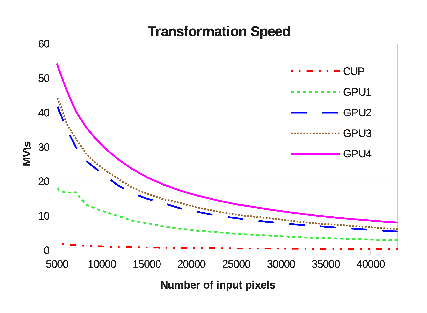
\includegraphics[scale=1.1]{part4/Laidler_O20/O20_f1} 
    \caption{Comparison of transformation speeds for the serial implementation (CPU) and four kernels (GPU1-4) on a  128x128x128x128 HS centered on $a=250 Hz \ b=0.5 Hz \ c=0.000196 \ d=1.445$ }  
    \label{speed}
  \end{subfigure}
  ~
  \begin{subfigure}[b]{0.45\textwidth}
    \centering
    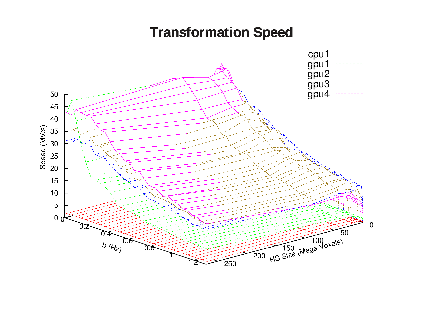
\includegraphics[scale=1.1]{part4/Laidler_O20/O20_f2}
    \caption{The effects of tile size and amplitude parameter on transformation speed, for tiles centered on $a=250 Hz \ c=0.000196 \ d=1.445$ and a rage of $b$ values.}
    \label{speed2}
  \end{subfigure}
  \caption{Transform Speeds}
\end{figure}

Fig.~\ref{speed} shows the transformation speeds for a sample tile, representing an average speedup of $9.73, 19.16, 20.66$ and $25.79$ for GPU1, GPU2, GPU3, and GPU4  kernels respectively. Two key factors affecting transformation speed are the amplitude parameters covered by a tile and the tile size (Fig.~\ref{speed2}). The amplitude coverage has two main effects firstly it influences the number of input pixels selected: lower $b$ values lead to fewer points requiring transformation and thus faster filling of a tile of a given size. The amplitude also affects the shape of the hyperplane: a large $b$ will amplify changes in $c$, which can be thought of as increasing the separation of the 3D planes. Interestingly, each of the kernels has combinations of the two factors for which it outperforms the other kernels. For example, the GPU1 kernel, which allocates one thread per input pixel, is the fastest for values of $b$ below $0.1$ where there are few input pixels and planes are close to parallel, giving the low divergence of GPU1 an advantage. However, larger $b$ values result in  calculation of many $a$ values that are are not in the HS and result in a rapid decrease in GPU1's performance.

For all transformation kernels except GPU2, larger tiles lead to higher speeds. GPU2 performs well when the tile dimensions ($p$ and $q$) are close to the CUDA thread block dimensions, or low multiples thereof. As threads are distributed across $p,q$ pairs, large tiles result in a low number of thread blocks in which all threads are active. The use of SM in GPU3 to precalculate and store the lookup buffer does not significantly improve results, as the method used to find the first $y$ value requires fewer cycles than the memory access required by the look-up method. For large tiles, GPU4 usually has the best performance, running  20 to 25 times faster than the serial CPU implementation. Here the SM is used to store the results of calculations involving complex trigonometric functions. With large tiles, there are enough active thread blocks to effectively hide shared memory access and synchronization. For all kernels, speeds flatten off once the hypercubes reach side lengths of $\sim$64, at which point the GPU is fully utilized.

\section{Conclusions}
\label{Conclusion}

We have demonstrated that our parallel GPU implementations of the 4D sinusoidal Hough Transformation significantly reduce transformation time by 20 to 25 times. As a general rule, it is best to use as large a tile size as possible. With GPU implementations, best results are obtained with the use of SM to store complex calculations and intelligent loop ordering to allow selection of applicable input pixels. In future work, we will discuss the power of these transforms for automated blind searching of binary pulsars.  

\bibliography{editor}
